\newSec[Test]{Software Tests}{1}
Es gibt folgende Test-Arten:
\begin{itemize}
\item Unit Test
\item Integration Test
\item System Test
\item Acceptance Test
\end{itemize}

Allerdings wird in dieser Ausarbeitung nur auf Unit Tests eingegangen.


\newSec[TestUnit]{Unit Tests}{2}
In dem betrachteten Code wurde auf das Google Test-Framework (\textit{gtest} und \textit{gmock}) zurückgegriffen. Hierbei handelt es sich um ein weitverbreitetes Test-Framework. 

Es wurde darauf geachtet, den produktiv-Code vom Test-Code zu tennen. Dies wurde durch verschiedene Projekte innerhalb einer \textit{MS Visual Studio Solution} umgesetzt.


\newSec[TestUnitUsed]{Umgesetzte Unit Tests}{3}
Als Nachweis über das Vorhandensein der Unit-Tests soll an dieser Stelle ein Verweis auf die jeweiligen .cpp-Dateien genügen. Diese sind durch ihren Inhalt für sich selbstsprechend. Wie allgemein wünschenswert: Alle Tests sind erfolgreich (siehe \refImg{fig:TestRes}).

\begin{itemize}
\item https://github.com/MobMonRob/ROSLabDrohne/blob/9edc7b5814c1bb731abf0f7af4352289e57b681f/Code/Test\_Domain/test.cpp
\item https://github.com/MobMonRob/ROSLabDrohne/blob/9edc7b5814c1bb731abf0f7af4352289e57b681f/Code/Test\_DroneController/test.cpp
\item https://github.com/MobMonRob/ROSLabDrohne/blob/9edc7b5814c1bb731abf0f7af4352289e57b681f/Code/Test\_Adapter/test.cpp
\item https://github.com/MobMonRob/ROSLabDrohne/blob/9edc7b5814c1bb731abf0f7af4352289e57b681f/Code/Test\_Controller/test.cpp
\item https://github.com/MobMonRob/ROSLabDrohne/blob/9edc7b5814c1bb731abf0f7af4352289e57b681f/Code/Test\_PlugIn/test.cpp
\end{itemize}
\missing[hier Links statt der kompletten URI]

\begin{figure}[ht!]
\vspace{0.25cm}
\begin{center}
\fbox{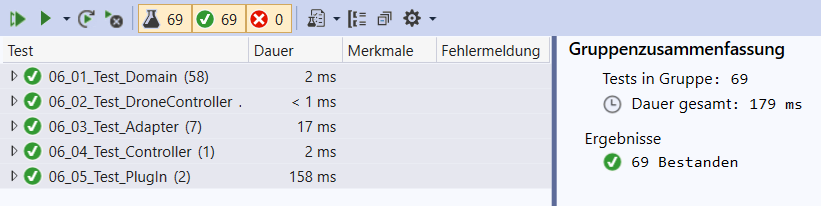
\includegraphics[width=15cm]{Pictures/Test Result.png}}
\caption{Ergebnisse der Unit-Tests}
\label{fig:TestRes}
\end{center}

\vspace{0.25cm}
\end{figure}


\newSec[TestUnitNorm]{AAA-Normalform}{4}
Der allgemeine Aufbau eines Unit-Tests, wie er auch in diesem Projekt angewandt wurde, wird hier anhand eines Beispiels (siehe \refImg{fig:TestAAA}) demonstriert.

\begin{figure}[ht!]
\vspace{0.25cm}
\begin{center}
\fbox{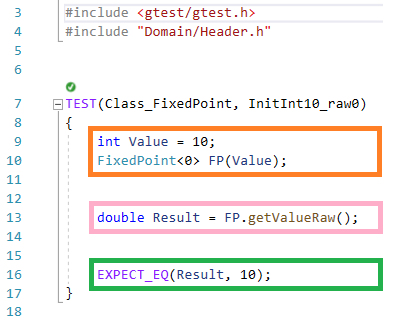
\includegraphics[width=12cm]{Pictures/Test AAA.png}}
\caption{AAA-Normalform an einem Beispiel-Test}
\label{fig:TestAAA}
\end{center}

\vspace{0.25cm}
oranger Kasten:	Arrage-Bereich\\
rosa Kasten: Act-Bereich\\
grüner Kasten: Assert-Bereich
\end{figure}



\newSec[TestUnitMock]{Mocks}{4}
Der in diesem Abschnitt beschriebene Test enthält ein Mock.
Hier wird sichergestellt, dass die \CodeClass{PoseController} nach der Berechnung der aktuellen Pose (Übergabe des Parameters in \CodeMeth{feedbackPose}) die \CodeMeth{transmitAction} der Implementierung der \CodeClass{Transmitable} aufruft.

https://github.com/MobMonRob/ROSLabDrohne/blob/9edc7b5814c1bb731abf0f7af4352289e57b681f/Code/Test\_Controller/test.cpp\#L15
\missing[hier Links statt der kompletten URI]

Ein Sonderfall ergibt sich für die \textit{Verify}-Phase des Mocks innerhalb des \textit{gmock}-Frameworks. Diese wird nicht benötigt:
\glqq instead of checking the system state at the very end, mock objects verify that they are invoked the right way and report an error as soon as it arises, giving you a handle on the precise context in which the error was triggered. This is often more effective and economical to do than state-based testing.\grqq \cite{gmockFAQ}


\newSec[TestUnitATRIP]{ATRIP-Regeln}{3}
\newSec[TestUnitATRIPAuto]{Automatic}{4}
Um diese Eigenschaft zu gewährleisten, wurden Parameter \textit{hard coded} in die Tests eingeführt (keine manuellen Interaktionen).
Im betrachteten Code war negativ-Beispiel auffindbar.


\newSec[TestUnitATRIPThor]{Thorough}{4}
Die Anforderungen an die Testbarkeit dieses Projekts halten sich in Grenzen. Daher ist davon auszugehen, dass große Teile der Funktionalität nicht durch Tests abgedeckt sind.\\
\note{In Zuge der \textit{TDD} Entwicklung der \CodeClass{FixedPoint<T>} wurde eine vollständige Testabdeckung gewährleistet (siehe \refCap{TDD}).}


\newSec[TestUnitATRIPRep]{Repeatable}{4}
Um diese Eigenschaft zu gewährleisten, wurden Parameter \textit{hard coded} in die Tests eingeführt (Kein Zufall, keine Abhängigkeit von externen/berechneten Parametern).
Durch den Einsatz eines Test-Frameworks können die Unit Tests jederzeit durchgeführt werden.


\newSec[TestUnitATRIPInd]{Independent}{4}
Tests wurden so geschrieben, dass sich diese nicht gegenseitig beeinflussen und jeweils nur einen Funktionlität abprüft.

Im Gegenzug wurden an diversen Stellen Tests für verschiedene parameter der selben Methode separat geschrieben. Hier würde beim Fehlerfall dieser Methode mehrere Tests scheitern.
\zB\ Abprüfen der \CodeMeth{getMedianState}:\\
https://github.com/MobMonRob/ROSLabDrohne/blob/9edc7b5814c1bb731abf0f7af4352289e57b681f/Code/Test\_Adapter/test.cpp\#L110
https://github.com/MobMonRob/ROSLabDrohne/blob/9edc7b5814c1bb731abf0f7af4352289e57b681f/Code/Test\_Adapter/test.cpp\#L139
https://github.com/MobMonRob/ROSLabDrohne/blob/9edc7b5814c1bb731abf0f7af4352289e57b681f/Code/Test\_Adapter/test.cpp\#L175
\missing[hier Links statt der kompletten URI]

Um die Debug-Tätigkeit zu vereinfachen, werden für einen Fehlerfall in aufwändigeren Tests menschenlesbare Informationen über die errechneten Ergebnisse zur Verfügung gestellt\footnote{Das eingesetzte Test-Framework zeigt hier lediglich den Speicherinhalt in hexadezimalem Format an.}. HIerdurch wird das Auffinden der Ursache des Fehlers erleichtert.

Die Nutzung von Mocks sorgt \ua\ für eine Unabhängigkeit von Fehlerfällen anderer Klassen durch ein definiertes Verhalten des Mocks für genau den Test, in dem dieser Mock trainiert wurde (siehe \refCap{TestUnitMock}).


\newSec[TestUnitATRIPProf]{Professional}{4}
Allgemein wurde versucht, die Lesbarkeit der Tests zu gewährleisten, indem kurze und aussagekräftig\footnote{\grq aussagekräftig\glq ist immer subjektiv} Tests geschrieben wurden.
Hierzu wurden die Abschnitte aus \refCap{TestUnitATRIP} mit doppelten Leerzeilen getrennt und zudem an geeigneten Stellen Leerzeilen zur Übersichtlichkeit eingefügt.

Leider konnte dies aufgrund der Komplexität des zu testenden Use Cases nicht immer eingehalten werden:
\zB\ https://github.com/MobMonRob/ROSLabDrohne/blob/9edc7b5814c1bb731abf0f7af4352289e57b681f/Code/Test\_Adapter/test.cpp\#L175 (Zeilenanzahl > 25 Zeilen)

\missing[hier Links statt der kompletten URI]





\newSec[TestCover]{Code Coverage}{3}


\missing[Reka fragen]


using \texttt{coverlet} with \texttt{Visual Studio}



\newSec[TestCoverStart]{Getting Started}{4}
\begin{itemize}
\item installiere Microsoft.NET.Sdk
\item installiere Microsoft.NET.Test.Sdk (NuGet.org)



\end{itemize}


using \texttt{Google Test} with \texttt{Visual Studio}





\newSec[TDD]{TDD}{2}

\textit{Test Driven Development} (\textit{TDD}) ist ein Prozess in der Software-Entwicklung, wonach jede Klasse \bzw\ Funktion im produktiven Code bereits im Vorfeld durch einen Test abgedeckt wird.

Hierbeit unterscheidet sich das \textit{TDD} von \textit{Test First} dadurch, dass \textit{TDD} lediglich jeweils einen Test vor dem produktiven Code liegt, wobei \textit{Test First} eine beliebige Anzahl an Tests bereitstellen kann, bevor produktiver Code entsteht. \missing[Quelle die letzte Vorlesung - Sem6 VL 3 oder so?]

Im zugrundeliegenden \texttt{git}-Repository wird die Entwicklung einer Klasse nach dem \textit{Test First}-Prinzip im \Branch{createFixedPoint} mit folgendem \Commit{} gestartet.
 \Commit{a4f9bd383c32a7d6d1b0be2319764a664199c2d2}

